
\begin{enumerate}
\item 
\question{If you have a $9\myvolt$ voltage source, a blue LED, and a $500\myohm$ resistor all in series, how much current is running through the LED?}
\solution{The current running through the LED is $0.0114\myamp$, or $11.4\mymamp$.}
\explanation{Blue LEDs have a $3.3\myvolt$ voltage drop.  Diode voltage drops are relatively fixed.  Therefore, in this circuit, there are $9 - 3.3 = 5.7\myvolt$ left to account for.  Using Ohm's Law, we can figure out the current based on our resistor:
\begin{align*}
I &= V / R \\
  &= 5.7 / 500 \\
  &= 0.0114 \myamp
\end{align*}
The current in the circuit is $0.0114\myamp$, or $11.4\mymamp$.
Since this is a series circuit, the amount of current going into each junction is the same as the amount going out, so the current is the same throughout the whole circuit.
Therefore, this is also the amount of current going through the LED.
}
\item 
\question{If you have a $3\myvolt$ voltage source and a red LED, what size resistor do you need to put in series with the LED to have it use $3\mymamp$ of current?}
\solution{$400\myohm$}
\explanation{A red LED will yield a $1.8\myvolt$ drop.  
Therefore, the amount of voltage left to account for is $3 - 1.8 = 1.2\myvolt$.  
If we want $3\mymamp$ of current, we have to first convert that to amps to use Ohm's Law.
$3\mymamp$ is the same as $0.003\myamp$.
Therefore, using Ohm's Law we can see that:
\begin{align*}
R &= V / I \\
  &= 1.2 / 0.003 \\
  &= 400\myohm
\end{align*}
We would need a $400\myohm$ resistor to limit the current to $3\mymamp$.
}
\item 
\question{If you have a $10\myvolt$ voltage source, a blue LED, a red LED, and a $200\myohm$ resistor all in series, how much current is running through the LEDs?}
\solution{$24.5\mymamp$}
\explanation{The red LED will yield a $1.8\myvolt$ drop, the blue LEDD will yield a $3.3\myvolt$ drop.  With a $10\myvolt$ source, that leaves $10 - 1.8 - 3.3 = 4.9\myvolt$ remaining to account for.
After that, we can use Ohm's Law to determine how much current the resistor will limit the circuit to:
\begin{align*}
I &= V / R \\
  &= 4.9 / 200 \\
  &= 0.0245\myamp
\end{align*}
Therefore, the circuit will have a $0.0245\myamp$ current going through it, or $24.5\mymamp$.
Since it is a series circuit, that is the same current running through all the components, so the LEDs will have the same amount of current as well.
}
\item 
\question{If I have a $12\myvolt$ voltage source, a blue LED, and a red LED, and the LEDs have a maximum current of $30\mymamp$ before it breaks and a minimum current of $1\mymamp$ before it turns on, what range of resistors can I put in series with the LEDs to get them to light up without breaking?}
\solution{This circuit requires a resistor between $230\myohm$ and $6,900\myohm$.}
\explanation{This is solved just like the other problems, but we will have to solve the problem twice.
We need to know both the resistor value for $1\mymamp$ as well as the resistor value for $30\mymamp$.
This is very similar to problems encountered in real life, as you will often have a variety of components, and you just need to know the range of which components will work and which ones will break things.

So, first we need to calculate the amount of voltage which will be dropped by the resistors.
Since the LEDs have a fixed voltage drop, we can just subtract them from the battery voltage---$1.8\myvolt$ for the red and $3.3\myvolt$ for the blue.
That leaves us with $12 - 1.8 - 3.3 = 6.9\myvolt$ remaining.

The LEDs require a minimum of $1\mymamp$ ($0.001\myamp$) to light up.  So let's solve for resistance using that value:
\begin{align*}
R &= V / I \\
  &= 6.9 / 0.001 \\
  &= 6,900\myohm
\end{align*}
Therefore, the largest resistor we can put in this circuit and have it light up is $6,900\myohm$.

On the other end, the maximum current that can flow without harming the LEDs is $30\mymamp$ ($0.03\myamp$).
Therefore, we need to solve for resistance using that value for the current:
\begin{align*}
R &= V / I \\
  &= 6.9 / 0.03 \\
  &= 230\myohm
\end{align*}
Therefore, the smallest resistor we can get away with is $230\myohm$.
That means that we must use a resistor between $230\myohm$ and $6,900\myohm$.
}
\item 
\question{In the circuit below, calculate the how much current flowing through each component and each component's voltage drop if R1 is $500\myohm$ (note that the diode is just a regular diode, not an LED). \\ 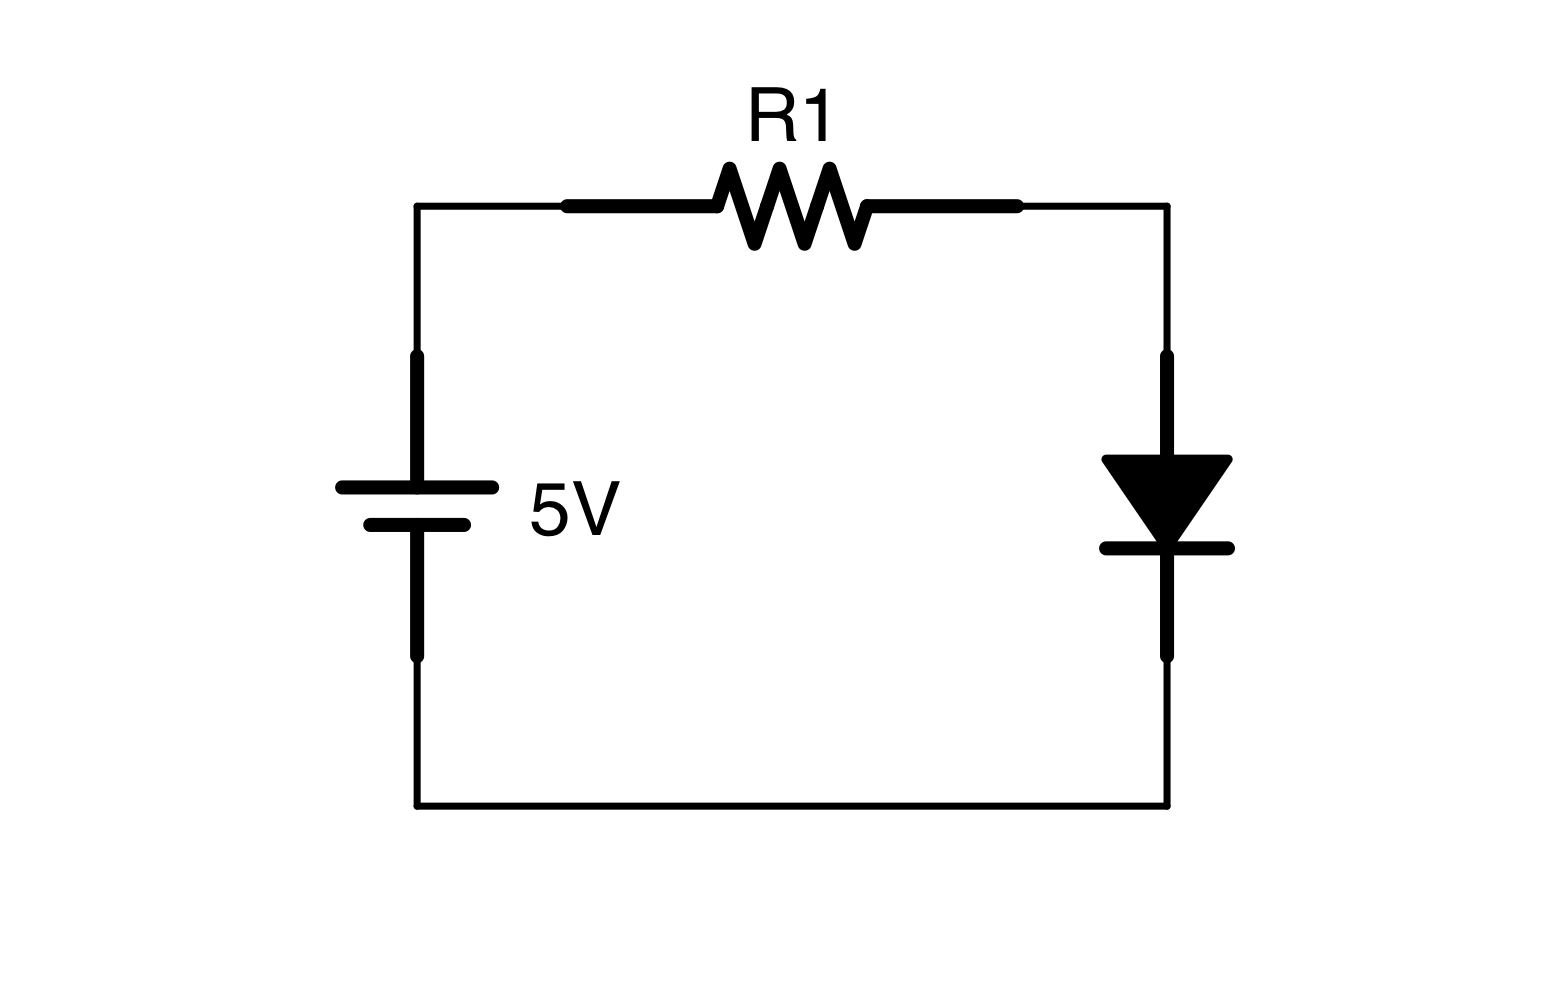
\includegraphics[width=\columnwidth]{DiodeApplyEx1.png}}
\solution{\begin{description}
\item[R1] $4.4\myvolt$ drop with $8.8\mymamp$ current
\item[Diode] $0.6\myvolt$ drop with $8.8\mymamp$ current
\end{description}}
\explanation{The total voltage drop for the circuit is $5\myvolt$ because that is the size of the battery.
The voltage drop across the diode is fixed at $0.6\myvolt$.
That means that the remaining voltage is dropped across the resistor, which will be $5 - 0.6 = 4.4\myvolt$.
We can use Ohm's Law to find the current flowing across the resistor:
\begin{align*}
I &= V / R \\
  &= 4.4 / 500 \\
  &= 0.0088 \myamp
\end{align*}
The current flowing through the resistor is $0.0088\myamp$, which is $8.8\mymamp$.
Since the circuit is a series circuit, this is the same current flowing through every component.
}
\item 
\question{Let's say instead of an ordinary diode, the diode is a blue LED.  Recalculate the current going through each component and the voltage drops for each component.}
\solution{\begin{description}
\item[R1] $1.7\myvolt$ drop with $3.4\mymamp$ current
\item[Diode] $3.3\myvolt$ drop with $3.4\mymamp$ current
\end{description}}
\explanation{With a blue LED, the voltage drop changes from $0.6\myvolt$ to $3.3\myvolt$.
This means that there is only $5 - 3.3 = 1.7\myvolt$ left to account for in the circuit (thus, dropped by the resistor).
Using Ohm's Law, we can calculate the current flowing through the resistor:
\begin{align*}
I &= V / R \\
  &= 1.7 / 500 \\
  &= 0.0034 \myamp
\end{align*}
Therefore, the current is $0.0034\myamp$ ($3.4\mymamp$) through the circuit.
}
\item 
\question{In the circuit below, calculate how much current is flowing through each component and each component's voltage drop if R1 is $300\myohm$, R2 is $400\myohm$, and R3 is $500\myohm$.  \\ 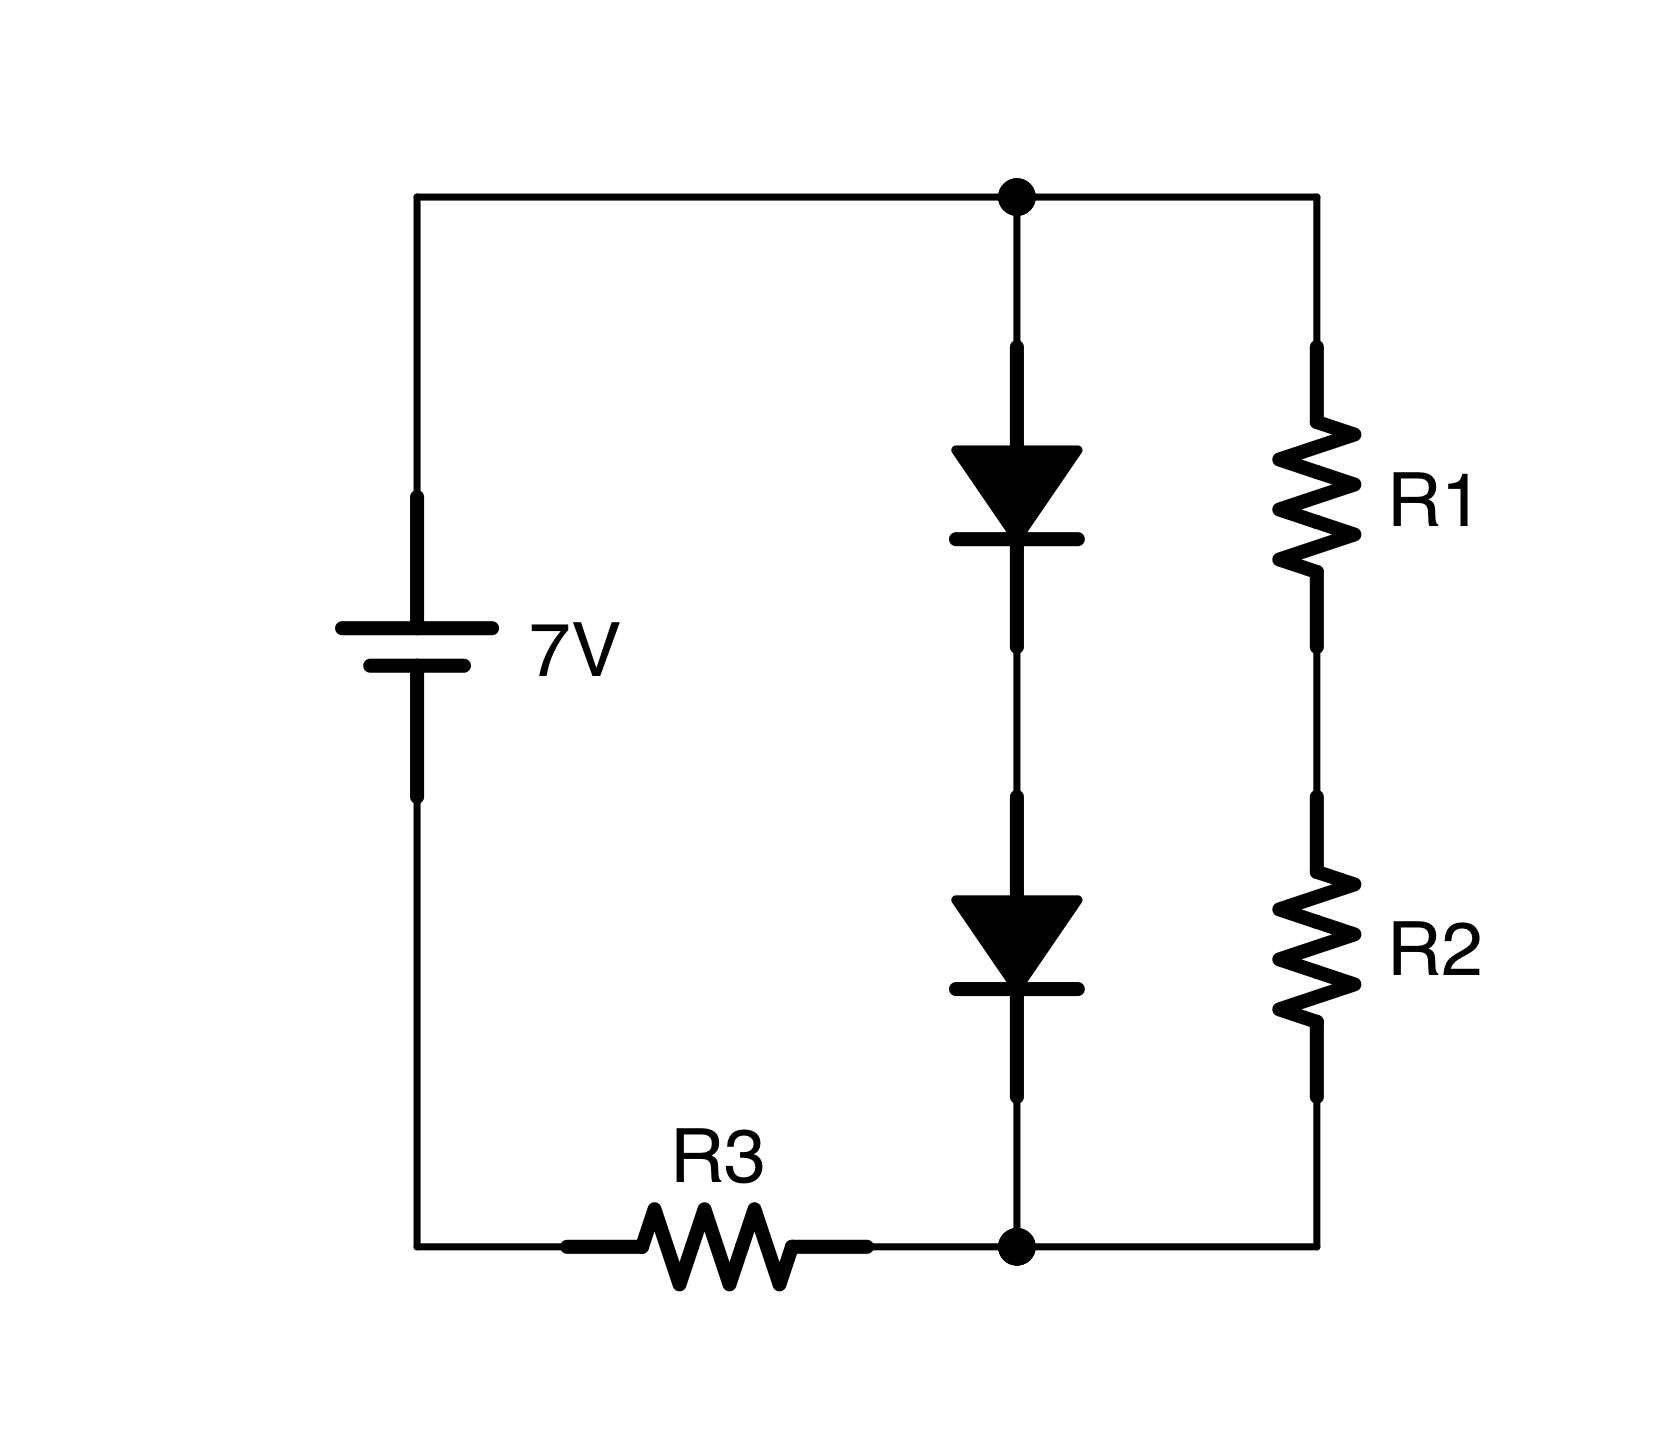
\includegraphics[width=\columnwidth]{DiodeApplyEx2.png}}
\solution{\begin{description}
\item[Diodes] Both diodes each have $0.6\myvolt$ drop with $9.89\mymamp$ current 
\item[R1] $0.513\myvolt$ drop with $1.71\mymamp$
\item[R2] $0.684\myvolt$ drop with $1.71\mymamp$
\item[R3] $5.8\myvolt$ drop with $11.6\mymamp$
\end{description}}
\explanation{Here the voltage source is $7\myvolt$.  
That means that the total voltage drop along any path from the positive to the negative is $7\myvolt$.
Additionally, the voltage drop down the center (the two diodes) is fixed at $0.6 + 0.6 = 1.2\myvolt$.
That means that both the center and the right side (R1 and R2) both have a $1.2\myvolt$ drop (because Kirchoff's Voltage law states that all paths must have the same voltage drop, and these paths both begin and end in the same place).
So, the remaining part of the circuit is R3, and there are $7 - 1.2 = 5.8\myvolt$ left to account for in the circuit.
This means the voltage drop across R3 must be $5.8\myvolt$.

To calculate the current running through R3 we use Ohm's Law:
\begin{align*}
I &= V / R \\
  &= 5.8 / 500 \\
  &= 0.0116\myamp
\end{align*}
Because all current has to flow through R3 to get back to the negative terminal, this is the total current in the circuit.

Now, to find the current on the right side of the circuit, we can use Ohm's Law again.
Since R1 and R2 are in series, their total resistance is $300 + 400 = 700\myohm$.
So, to find the current:
\begin{align*}
I &= 1.2 / 700 \\
  &= 0.00171\myamp
\end{align*}
Therefore, the rest of the current has to be flowing through the diodes across the middle:
$$ 0.0116 - 0.00171 = 0.00989\myamp $$
The voltage drop for each resistor can be done with Ohm's Law:
\begin{align*}
V_{R1} &= I * R \\
       &= 0.00171 * 300 \\
       &= 0.513\myvolt \\
V_{R2} &= I * R \\
       &=  0.00171  * 400 \\
       &= 0.684
\end{align*}
This doesn't exactly add up to $1.2\myvolt$ because of rounding issues.
}
\item 
\question{Draw a circuit that provides a 6-volt regulated power supply to circuit load from a 9-volt battery using regular diodes.  Choose a resistor that works efficiently for a circuit load of $500\myohm$ and operates with a battery voltage from $7\myvolt$ to $9.6\myvolt$.  What is the current at the lowest and highest ranges of the battery?  How much is used by the circuit load and how much is wasted through the diodes in each configuration?}
\solution{The circuit below utilizes $13.3\mymamp$ at the lowest battery level, and $48\mymamp$ at the highest.  The circuit load will always utilize $12\mymamp$, and the rest of the current will be wasted through the diodes.
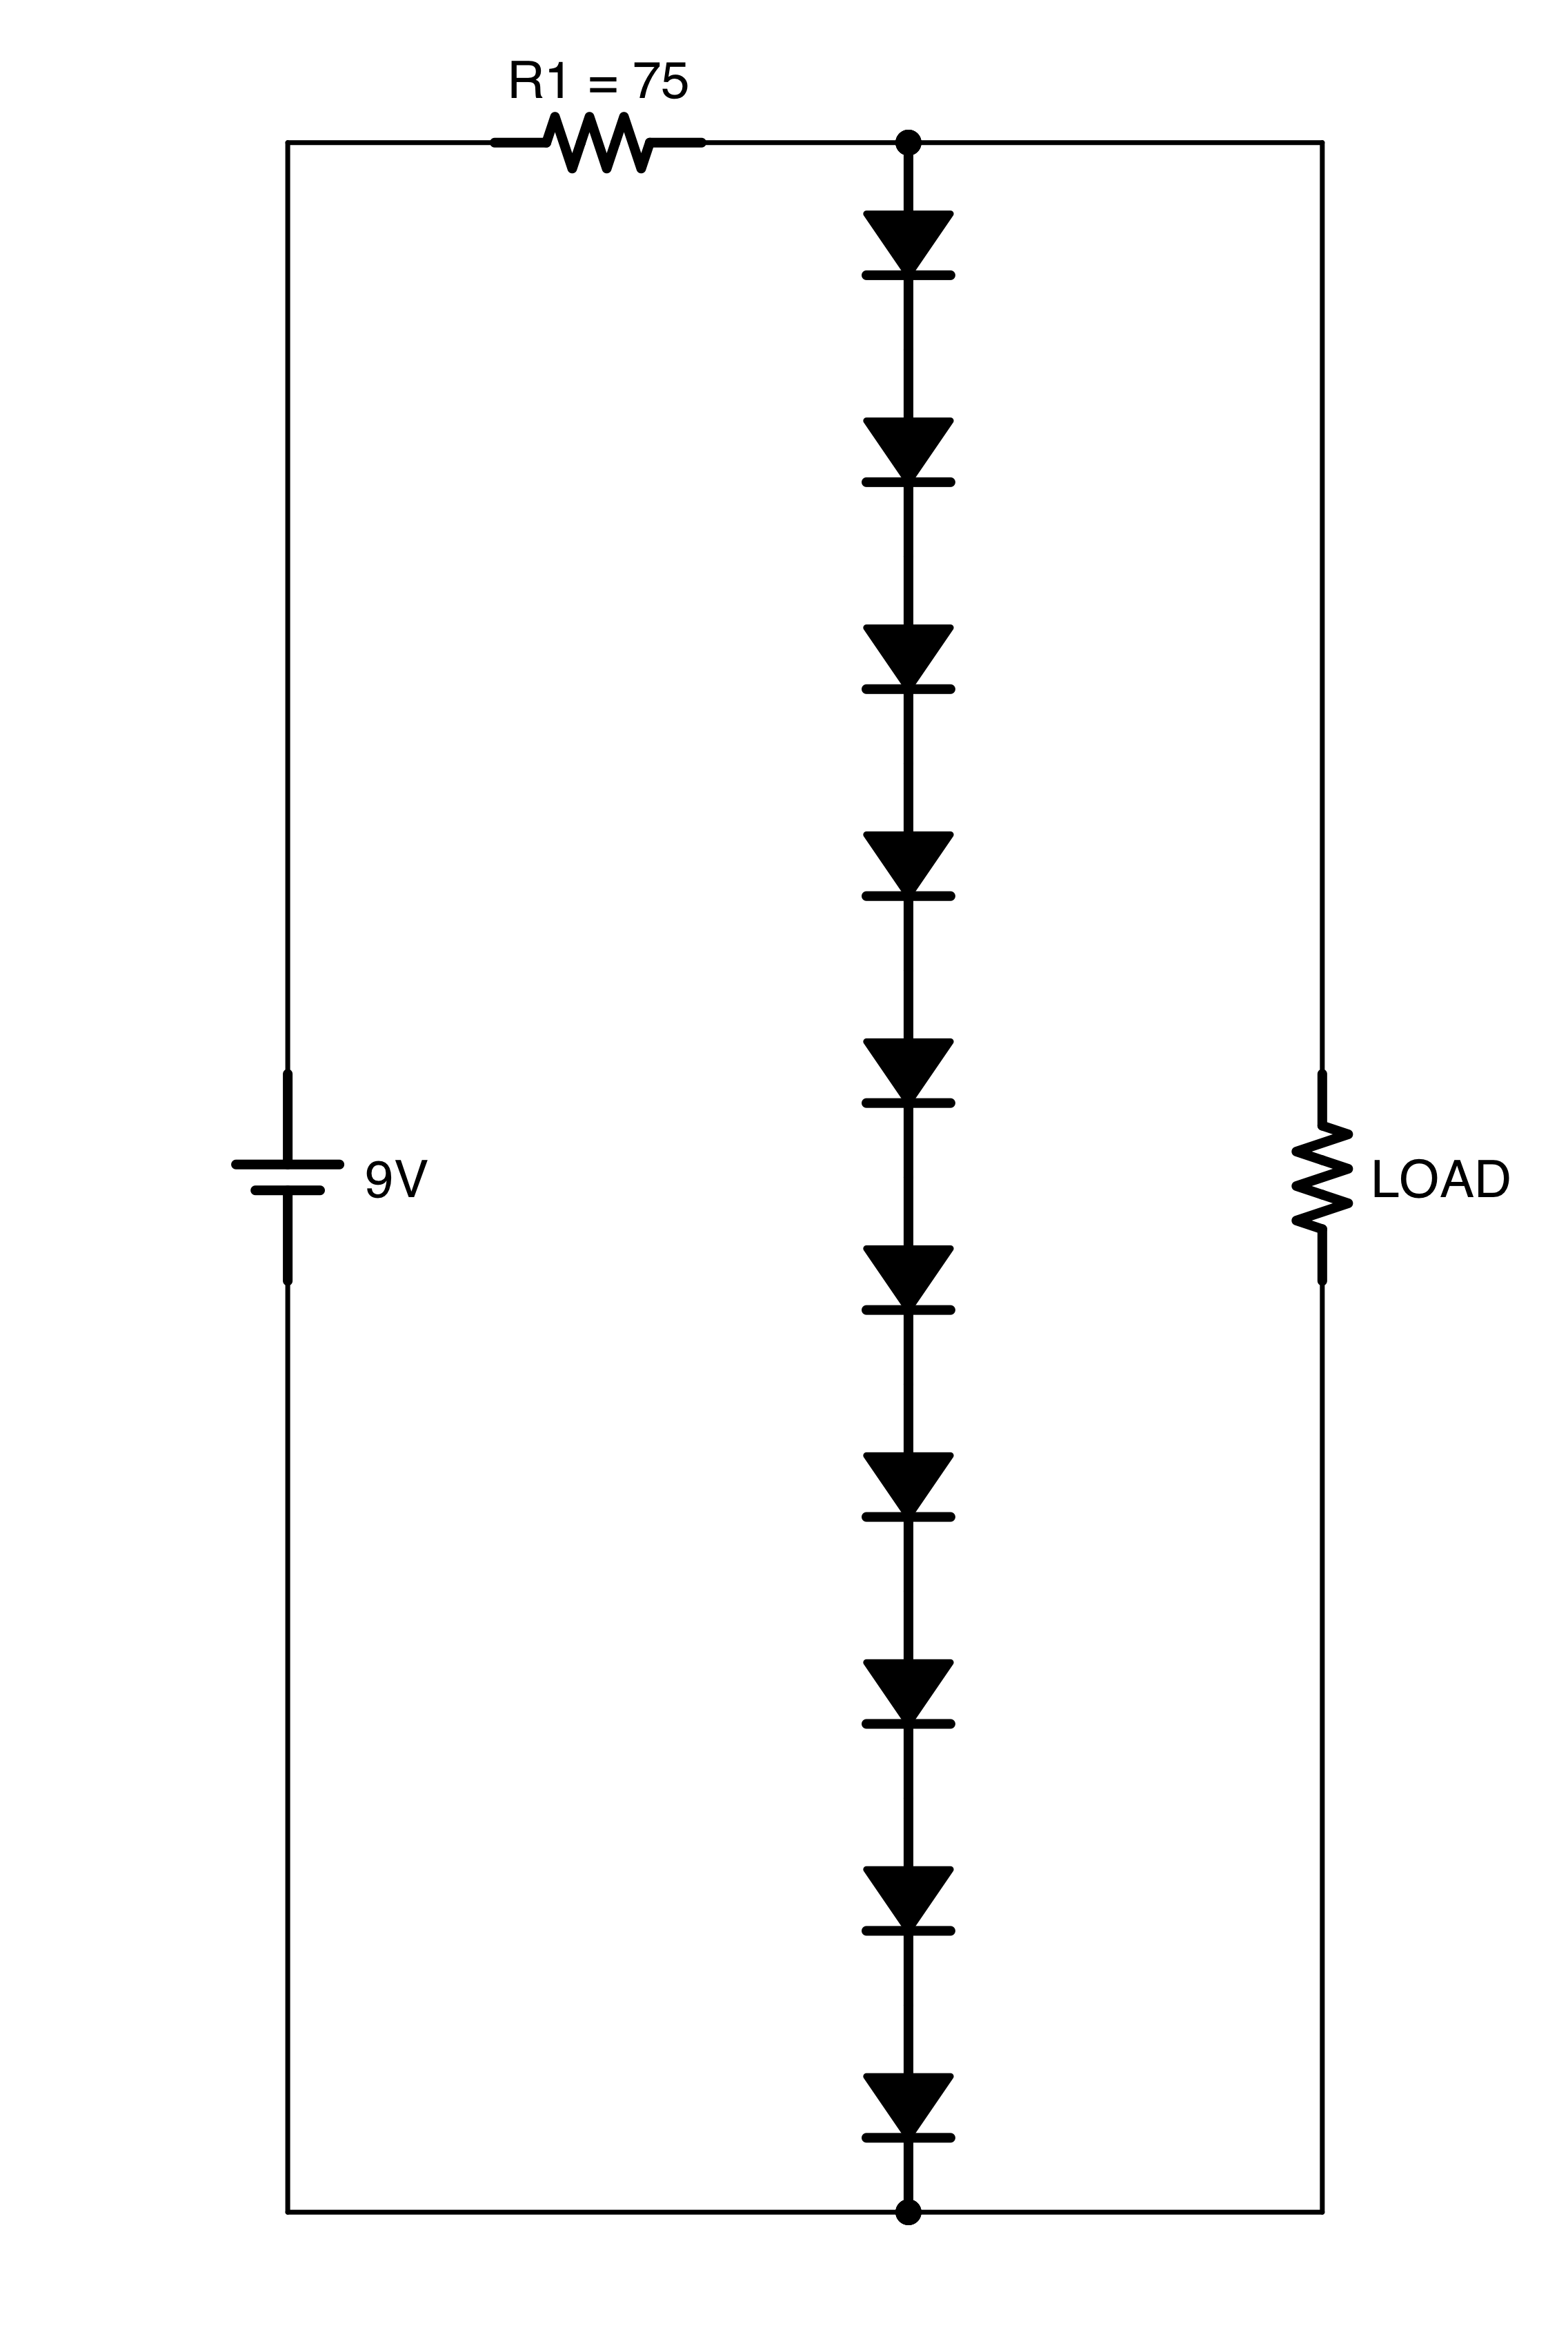
\includegraphics[width=\columnwidth]{DiodeExerciseVoltageReg.png}
}
\explanation{If the circuit load is $500\myohm$ with $6\myvolt$, then the current supplied can be calculated with Ohm's Law:
\begin{align*}
I &= V / R \\
  &= 6 / 500 \\
  &= 0.012\myamp
\end{align*}
We need this voltage drop to be fixed (that's what the problem states), so we will run diodes in parallel.
This will fix the voltage drop across the load.
Since each diode drops $0.6\myvolt$, we just need to supply 10 diodes in parallel with our load to ensure a $6\myvolt$ drop.

Now, the battery itself will supply more than $6\myvolt$, so we need an additional resistor either before or after the diode drop to mop up the extra voltage.
If the resistor is too small, a lot of current will be wasted (and, as we will see in later chapters, could cause the resistor to burn up).
If the resistor is too large, then the current will be too low to provide the power needed.
There will always bee some wasted current (this current will flow through the diode bridge), but the goal is to keep it to a minimum.

If we decided to allow a $1\mymamp$ current go through the bridge at the lowest battery voltage (this is somewhat arbitrary, but $1\mymamp$ is a workable amount of waste current), then we can calculate the resistor we need using Ohm's law.
We said that the lowest battery setting we would consider is $7\myvolt$, which leaves $1\myvolt$ left over.

Since the current that needs to flow through the circuit is $0.012\myamp$, and we want a $1\mymamp$ ($0.001\myamp$) headroom, that means that the current going through the resistor will be $0.013\myamp$.
So the resistor will be:
\begin{align*}
R &= V / I \\
  &= 1 / 0.013 \\
  &= 76.92 \\myohm
\end{align*}
You might round this down to whatever value of resistor you have (you want to round down because rounding up could limit the current too much).
I have a $75\myohm$ resistor in my collection, so we will work with that.

So, with a $75\myohm$ resistor, we can calculate the current flowing at each configuration---the battery at $7\myvolt$ and at $9.6\myvolt$.
Since the circuit load is fixed at $6\myvolt$, that means that the current flowing through the resistor will be $7 - 6 = 1\myvolt$ and $9.6 - 6 = 3.6\myvolt$, respectively.

So, the current at $6\myvolt$ is:
\begin{align*}
I &= V / R \\
  &= 1 / 75 \\
  &= 0.0133\myamp = 13.3\mymamp
\end{align*}
Since the circuit is using $12\mymamp$ this circuit wastes $1.3\mymamp$.

At $9.6\myvolt$ the current will be:
\begin{align*}
I &= V / R \\
  &= 3.6 / 75 \\
  &= 0.048\myamp = 48\mymamp
\end{align*}
Since the circuit uses $12\mymamp$, this circuit wastes $36\mymamp$.

Your circuit design may be slightly different based on how much current you were willing to waste, but the important part is to calculate that the load will need $12\mymamp$, to figure out a ``reasonable'' resistor value, and to calculate how much current is wasted in each battery level.
}
\item 
\question{Draw an equivalent circuit to the previous question using a Zener diode instead of normal diodes.}
\solution{

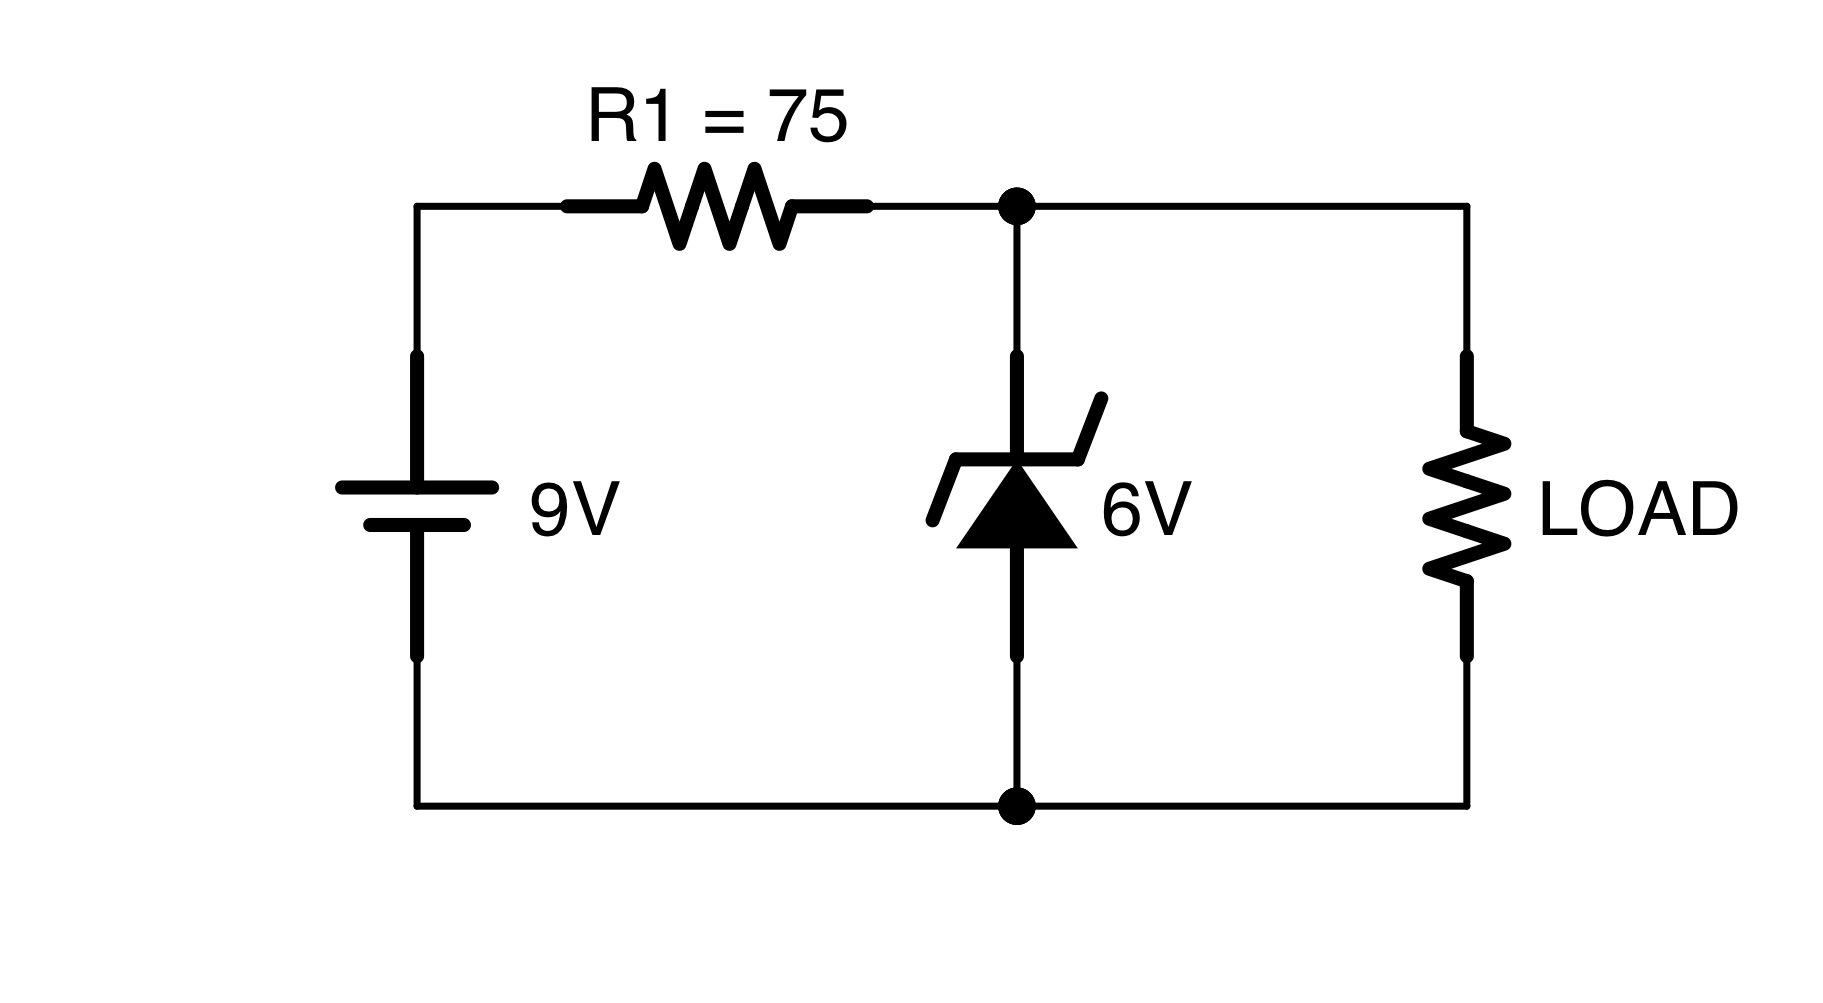
\includegraphics[width=\columnwidth]{DiodeExerciseVoltageRegZener.png}}
\explanation{This is the same circuit, but with the individual diodes replaced with a single Zener diode of the proper voltage.  Because we use the breakdown voltage of the Zener rather than the forward voltage drop, it is wired ``backwards'' in the circuit.}
\end{enumerate}
